\chapter{Rigid Fluid Coupling}
\label{chap:rfc}

\section{Introduction}
\label{sec:rfc:intro}
In the current chapter, we model the dynamics of rigid bodies in fluid flow and
the coupled behavior of fluid and rigid bodies. Transport of arbitrarily shaped
rigid bodies in fluid flows is a common phenomenon that occurs widely in nature.
The transport of bodies in internal systems \parencite{Dai2021}, debris flow
\parencite{Qingyun2022}, the food processing industry \parencite{Karunasena2014}, and
ice-sea modeling \parencite{Mintu2018} are a few areas to mention. These systems are
studied as part of two-way coupling models. The two-way coupling phenomena are
nonlinear, and an analytical study is not feasible. A numerical study is
preferable while handling such a phenomenon. A mesh-based or meshless technique
can be utilized to study rigid fluid coupling (RFC) numerically.


In the current chapter, we couple CTVF with DEM to handle the rigid fluid
coupling problems. The fluid is modeled using a corrected transport
velocity formulation developed in \cref{chap:ctvf}. CTVF provides smooth
pressure distribution with EDAC formulation and homogeneous particle
distribution, resulting in accurate fluid modeling. Rigid-rigid interactions are
modeled with DEM. The interaction between the fluid and rigid bodies is
handled using the dummy particle approach \parencite{Adami2012}.
% We explore different rigid fluid coupling strategies by simulating high
% density ratio simulations.


\FloatBarrier%
\section{Numerical Methodology}
\label{sec:rfc:rbd}
% The rigid body is discretized into particles with equal spacing each particle
% with mass $m_i$ and density $\rho_i$. Rigid body has a total 6 degrees of
% freedom (DOF), divided into $3$ translational and $3$ rotational.
The equations governing the dynamics of a rigid body are, balance of linear and
angular momentum given by,
\begin{equation}
  \label{eq:rfc:balance_linear_mom}
  \frac{d \; (M \ten{v}_{cm})}{d t} = \sum_i \ten{F}_i,
\end{equation}
\begin{equation}
  \label{eq:rfc:balance_angular_mom}
  \frac{d \ten{L}}{d t} = \teng{\tau}_{cm},
\end{equation}
where $M$, $\ten{v}_{cm}$ are the mass and velocity of the center of mass of the rigid body.
$\ten{F}_i, \teng{\tau}_{cm}, \ten{L} $ are force acting at point $i$, torque and
angular momentum about the center of mass of the rigid body. In the current
case, force acting on the particle $i$, $\ten{F}_i$, is due to the interaction
with the other bodies and with the fluid particles, and any other body forces.
The torque $\teng{\tau}_{cm}$ and angular momentum $\ten{L}$ are computed as,
\begin{equation}
  \label{eq:rfc:torque}
 \teng{\tau}_{cm} = \sum_i \ten{F}_i \times (\ten{x}_{cm} - \ten{x}_{i}),
\end{equation}
\begin{equation}
  \label{eq:rfc:moi}
  \teng{L} =
  \sum_i \; \ten{r}_i \times \; (\teng{\omega} \times \ten{r}_i)
  = \sum_i \; m_i \; [(\ten{r}_i \cdot \ten{r}_i) \ten{I} - \ten{r}_i \otimes \ten{r}_i].
\end{equation}
Here $\ten{x}_{cm}$ and $\omega$ are the position of the center of mass and
angular velocity of the rigid body. $m_i$, $\ten{x}_{i}$, $\ten{r}_i$ are the
mass, position of particle, and position of particle $i$ with respect to vector
center of mass.

\begin{figure}[!htpb]
  \centering
  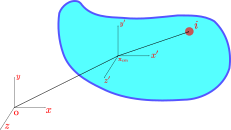
\includegraphics[width=0.7\textwidth]{images/rfc/images/rigid_body/rigid_body}
  \caption{Body frame and local frame description of rigid body}
  \label{fig:gloabl_body_frame_rb}
\end{figure}
We use two coordinate frames to capture the dynamics of the rigid body, a
global frame and a body frame as shown in
\cref{fig:gloabl_body_frame_rb}. The body fixed frame, which moves with
rigid body is always located at the center of mass ($\ten{x}_{cm}$). The
state of the rigid body at a given time ($t$) can be described using position
($\ten{x}_{cm}$) and velocity ($\ten{v}_{cm}$) of the center of mass, a
rotation matrix($\ten{R}$) to represent the orientation of the rigid body with
respect to the global frame, and angular velocity($\teng{\omega}$). The center
of mass is computed as
\begin{equation}
  \label{eq:rfc:center_of_mass}
  \ten{x}_{cm} = \frac{\sum_i m_i \; \ten{x}_{i} }{\sum_i m_i }.
\end{equation}
The position of the discretized particle ($i$) in
\cref{fig:gloabl_body_frame_rb} belonging to the rigid body at time $t$ can be
computed as,
\begin{equation}
  \label{eq:rfc:rb_particle_pos_update}
  \ten{x}_i = \ten{x}_{cm} + \ten{r}_{i},
\end{equation}
with
\begin{equation}
  \label{eq:rfc:rb_particle_pos_update}
  \ten{r}_i = \ten{R} \overline{\ten{r}}_{i}.
\end{equation}
Here $\overline{\ten{r}}_{i}$ is the position of the particle $i$ about the body
frame axis and remains constant through out the simulation. The rotation matrix
$\ten{R}$ is used to bring the body frame position vector to the global frame
$\ten{O}$. Similarly the velocity vector is computed as,
\begin{equation}
  \label{eq:rfc:rb_particle_vel_update}
  \ten{v}_i = \ten{v}_{cm} + \teng{\omega} \times \ten{r}_{i}.
\end{equation}

We evolve the state of the rigid body through the integration of the
\cref{eq:rfc:balance_linear_mom,eq:rfc:balance_angular_mom}. The linear velocity of the
center of mass ($\ten{v}_{cm}$) and angular momentum ($\ten{L}$) at the next
timestep are computed as,
\begin{equation}
  \label{eq:rfc:lin_vel_cm_update}
  \ten{v}_{cm}^{n+1} = \ten{v}_{cm}^{n} + \frac{\ten{F}_{cm}}{M} \; \Delta t,
\end{equation}
\begin{equation}
  \label{eq:rfc:ang_mom_update}
  \ten{L}^{n+1} = \ten{L}^{n} + \teng{\tau}_{cm} \; \Delta t.
\end{equation}
Here, $\ten{F}_{cm} = \sum_i \ten{F}_i$.

The position of the center of mass and the rotation matrix ($\ten{R}$) are updated
by,
\begin{equation}
  \label{eq:rfc:lin_pos_cm_update}
  \ten{x}_{cm}^{n+1} = \ten{x}_{cm}^{n} + \ten{v}_{cm}^{n} \; \Delta t,\\
  \ten{R}^{n+1} = \ten{R}^{n} + \tilde{\teng{\omega}}^{n} \, \ten{R}^{n} \; \Delta t,
\end{equation}
where $\tilde{\teng{\omega}}^{n}$ is matrix formulation of angular velocity
$\omega$. The angular velocity at the new time step is computed with
\begin{equation}
  \label{eq:rfc:ang_velocity_update}
  \teng{\omega}^{n+1} = (\textit{\teng{I}}^{-1})^{n+1} \; \ten{L}^{n+1}.
\end{equation}
Here, moment of inertia at the new time step is computed as,
\begin{equation}
  \label{eq:rfc:moi_update}
  (\textit{\teng{I}}^{-1})^{n+1} = \ten{R}^{n+1} \textit{\teng{\overline{I}}}^{-1} (\ten{R}^{n+1})^T.
\end{equation}
where moment of inertia ($\textit{\teng{\overline{I}}}^{-1}$) in body frame is
used to compute in global frame at every time instant for faster computations.
The moment of inertia ($\textit{\teng{\overline{I}}}$) is computed as,
\begin{equation*}
\textit{\teng{\overline{I}}} =
\begin{bmatrix}
\sum_i m_i (y_i^2 + z_i^2) & -\sum_i m_i x_iy_i & -\sum_i m_i x_iz_i\\
-\sum_i m_i x_iy_i & \sum_i m_i (x_i^2 + z_i^2) &  -\sum_i m_i y_iz_i\\
-\sum_i m_i  x_iz_i & -\sum_i m_i y_iz_i & \sum_i m_i (x_i^2 + y_i^2)
\end{bmatrix}.
\end{equation*}

The position and velocity of the particles of the rigid body are updated by
\begin{eqnarray}
  \label{eq:rfc:rb_particle_pos_update}
  \ten{r}_i = \ten{R} \cdot \overline{\ten{r}}_{i},\\
  \ten{x}_i = \ten{x}_{cm} + \ten{r}_{i},\\
  \ten{v}_i = \ten{v}_{cm} + \teng{\omega} \times \ten{r}_{i}.
\end{eqnarray}

The force acting on particle $i$ is composed of interaction with the other rigid
bodies, and the fluid, given as
\begin{eqnarray}
  \label{eq:rfc:rb_particle_pos_update}
  \ten{F}_i = \ten{F}_{\text{Fl}}^i + \ten{F}_{\text{cont}}^i
\end{eqnarray}
We follow \cref{sec:contact-algorithm} to compute force
$\ten{F}_{\text{cont}}^a$ acting on particle $i$ due to the interaction with
the rigid bodies. The force $\ten{F}_{\text{Fl}}^i$ acting due to the
interaction with the fluid particles follows \cref{subsec:fsi}.

We model the fluid with the CTVF \parencite{adepu2021corrected} scheme
developed in \cref{chap:ctvf}. Similar to the fluid modeling in
\cref{chap:fsi}, we modify the momentum equation to include the force acting due
to the interaction with a solid body. The discretized momentum equation of the
fluid particle including the interaction force is given as
\begin{multline}
  \label{eq:rfc:sph-momentum-fluid}
  \frac{\tilde{d}\ten{u}_{a}}{dt} = - \sum_{b} m_b \bigg[
  \bigg(\frac{p_a}{\rho_a^2} + \frac{p_b}{\rho_b^2}\bigg) \ten{I} -
  \bigg(\frac{\ten{A}_a}{\rho_a^2} + \frac{\ten{A}_b}{\rho_b^2}
  \bigg) \bigg]
  \cdot \nabla_{a} W_{ab} \\
  + \ten{u}_{a} \sum_{b} \frac{m_b}{\rho_{b}} \; \tilde{\ten{u}}_{ab} \cdot
  \nabla_{a} W_{ab} + \sum_{b} m_b \frac{4 \eta \nabla W_{ab}\cdot
    \ten{r}_{ab}}{(\rho_a + \rho_b) (r_{ab}^2 + 0.01 h_{ab}^2)} \ten{u}_{ab} +
  \ten{g}_{a} + \frac{\ten{F}^a_{\text{Fl}}}{m_a}.
\end{multline}
The particles are transported with a transport velocity as described in
\cref{chap:ctvf,chap:fsi}. The boundaries are handled using the dummy particle
approach as described in \cref{chap:ctvf}.

\subsection{Time Integration}

Rigid body and the fluid follow the kick-drift-kick time integration scheme. The
modeling of rigid-rigid interaction requires lower time step than the fluid. We
choose the minimum of both the timesteps to move the system forward in time. For
the numerical stability of fluid, the time step depends on the CFL condition as,
\begin{equation}
  \label{eq:rfc:time-step-cfl}
  \Delta t_{\text{fluid}} = \mathrm{min} \bigg( 0.25 \; \frac{h}{c + |U|} ,  0.25 \; \frac{h^2}{\nu},  0.25 \; \frac{h^2}{g} \bigg),
\end{equation}
where $|U|$ is the maximum velocity magnitude, $c$ is the speed of sound
typically chosen as $10 |U|$ for fluids in this work. For rigid body, the time
step is constrained as,
\begin{equation}
  \label{eq:rfc:time-step-body-force}
  \Delta t_{\text{rb}} \leq \frac{\pi}{50} \sqrt{\frac{m}{K_r}}.
\end{equation}
A minimum timestep is chosen as
\begin{equation}
  \label{eq:rfc:time-step-body-force}
  \Delta t = min(\Delta t_{\text{fluid}}, \Delta t_{\text{rb}}).
\end{equation}



\FloatBarrier%
\section{Results and Discussion}
\label{sec:rfc:results}
In the current section we validate the developed schemes. We first, validate the
DEM model by simulating, rolling, sliding and collapse of rigid bodies. Falling
and rising of bodies in hydrostatic tank are considered to validate the coupled
model. All the results are fully automated with the automan package
\parencite{automan2018} and made fully reproducible. The source code for all the
problems demonstrated in this manuscript is made available at
\url{https://github.com/dineshadepu/rfc}.


\FloatBarrier%
\subsection{Cylinder Rolling on an Inclined Plane}
\label{sec:cylinder-rolling-on-an-inclined-plane}
A cylinder of diameter $1.0$ m rolling on an inclined plane under gravity is
simulated in the current test case. The physical model is shown in
\cref{fig:circular-body:schematic-1}, while the computational model is in
\cref{fig:circular-body:schematic-2}. In the computational model the $x$-axis
points in the direction of the slope, where the gravity makes an angle
$\theta=\frac{\pi}{3}$ with the vertical. The physical and the numerical
parameters are given in \cref{tab:circular-body-rolling-params}. A total of two
friction coefficients are considered. A rigid disk can roll and stick or slip
depending on the angle of inclination $\theta$ of the plane and the friction
coefficient between the bodies. Analytical expression of the variation of the
center of mass of the cylinder with time covering the stick or slip regimes is
given as
\begin{align}
  \label{eq:rfc:analytical-x-cm-rolling-cylinder}
  x_{cm}(t) =
  \begin{cases}
  x_0 + \frac{1}{2} \, g \, t^2 \, (\sin(\theta) - \mu \cos(\theta)) & \tan{\theta} > 3.5\mu \text{ (slip)}\\
  x_0 + \frac{1}{3} \, g \, t^2 \, \sin(\theta) & \tan{\theta} \leq 3.5\mu \text{ (stick)}
\end{cases}
\end{align}
Here, $x_0$ is the initial position of the center of mass of the cylinder. The
analytical expression, \cref{eq:rfc:analytical-x-cm-rolling-cylinder}, is used
to compare with the current numerical solver.
\begin{figure}[!htpb]
  \centering
  \begin{subfigure}{0.48\textwidth}
    \centering
    \includegraphics[width=0.5\textwidth]{images/rfc/images/de_2021_cylinder_rolling_on_an_inclined_plane/schematic_1}
    \subcaption{}\label{fig:circular-body:schematic-1}
  \end{subfigure}
  \begin{subfigure}{0.48\textwidth}
    \centering
    \includegraphics[width=0.7\textwidth]{images/rfc/images/de_2021_cylinder_rolling_on_an_inclined_plane/schematic_2}
    \subcaption{}\label{fig:circular-body:schematic-2}
  \end{subfigure}
  \caption{A (a) physical and (b) computational model of the rolling cylinder on a
    plane inclined at an angle $\theta$.}
\label{fig:circular-body-schematic}
\end{figure}
\begin{table}[!ht]
  \centering
  \begin{tabular}[!ht]{ll}
    \toprule
    Quantity & Values\\
    \midrule
    $\rho$, density & $2700$ kg\,m\textsuperscript{-3} \\
    $\mu$, friction coefficient & $0.3$ \& $0.6$ \\
    Time of simulation & $0.6$ s \\
    Resolution, $\delta x$ & $0.0025$ m\\
    Smoothing length factor, $h/\Delta x$ & 1\\
    gravity $[g_x, g_y, g_z]$ & $[g\,\sin(\theta), g\,\cos(\theta), 0.0]$\\
    $k_r$, Repulsive stiffness coefficient & $1e7$ \\
    $k_f$, Repulsive stiffness coefficient & $1e5$ \\
    % $\alpha_{damp}$ & 0.\\
    \bottomrule
  \end{tabular}
  \caption{Material properties and numerical parameters used for the rolling
    of cylinder on an inclined surface.}%
  \label{tab:circular-body-rolling-params}
\end{table}

\Cref{fig:cylinder-xcom-vs-time} depicts the variation of center of mass of
the cylinder with time for friction coefficients $0.3$ and $0.6$,
respectively. From the \cref{fig:cylinder-xcom-vs-time} we can see that the
current solver matches well with the analytical solution.
\begin{figure}[!htpb]
  \centering
  \includegraphics[width=0.6\textwidth]{figures/rfc/figures/de_2021_cylinder_rolling_on_an_inclined_plane_2d/xcom_vs_time}
  \caption{x-component of center of mass variation with time for a cylinder
    rolling down an inclined plane.}
\label{fig:cylinder-xcom-vs-time}
\end{figure}


\FloatBarrier%
\subsection{Rigid Body Sliding Down an Inclined Plane}
\label{sec:rigid-body-sliding}
In this test case, free sliding of a rigid cube on a frictional inclined plane
is studied. The frictional part of the current solver is validated through this
test. The velocity of the center of mass of the cube is compared against the
analytical solution for quantitative validation. The schematic is shown is
\cref{fig:rigid_body_sliding}.
\begin{figure}[!htpb]
  \centering
  \includegraphics[width=0.4\textwidth]{images/rfc/images/rigid_body_sliding/schematic}
  \caption{Schematic of a square body sliding down an inclined plane under gravity.}
\label{fig:rigid_body_sliding}
\end{figure}
The rigid body of length $0.1$ m, height $0.1$ m, is allowed to slide on a
frictional surface which is at an angle $\frac{\pi}{3}$. A density of $2000$
kg\,m\textsuperscript{-3} is used for the body. Other numerical parameters, such
as the repulsive spring stiffness $k_r=3.0 \times 10^{5}$ $N/m$ and tangential
spring stiffness $k_t=3.0 \times 10^{5}$ $N/m$ is chosen, respectively. A
particle spacing of $0.01$ m is considered, resulting in $120$ particles in
rigid body discretization. From the analytical solution, the evolution of
velocity is given by,
\begin{equation}
  \label{eq:rfc:ce}
  \ten{v}(t) = (\mu \teng{g} \sin (\theta) - \teng{g} \cos (\theta)) t.
\end{equation}
We have considered three different friction coefficients, $\mu=0.2$,
$0.3$, and $0.6$. From the analytical solution, when the friction
coefficient is greater than $\tan(\frac{\pi}{3})$, we have no slip condition
and the body doesn't slide.

% \subsubsection{2D sliding}
% \label{sec:results-2d-sliding}
\Cref{fig:mohseni-2021-sliding-2d} shows the snapshots of the rigid body at
three time instants. From \cref{fig:mohseni-2021-sliding-2d} we can see that
the the body is freely sliding with out having any oscillations or unphysical
jumping off the inclined wall. This is because of the new surface aware
contact model as force is not computed by considering the wall as spherical
\begin{figure}[!htpb]
  \centering
  \begin{subfigure}{0.48\textwidth}
    \centering
    \includegraphics[width=1.0\textwidth]{figures/rfc/figures/mohseni_2021_free_sliding_on_a_slope_2d/fric_coeff_0_2/time0}
    \subcaption{t = $0$ s}\label{fig:passing-0}
  \end{subfigure}
  %
  \begin{subfigure}{0.48\textwidth}
    \centering
    \includegraphics[width=1.0\textwidth]{figures/rfc/figures/mohseni_2021_free_sliding_on_a_slope_2d/fric_coeff_0_2/time1}
    \subcaption{t = $0.5$ s}\label{fig:passing-1}
  \end{subfigure}

  \begin{subfigure}{0.48\textwidth}
    \centering
    \includegraphics[width=1.0\textwidth]{figures/rfc/figures/mohseni_2021_free_sliding_on_a_slope_2d/fric_coeff_0_2/time2}
    \subcaption{t = $1$ s}\label{fig:passing-2}
  \end{subfigure}
  \caption{Snapshots of rigid body sliding down an inclined plane with a
    friction coefficient of $0.2$.}
\label{fig:mohseni-2021-sliding-2d}
\end{figure}
particles but by the method discussed in \cref{sec:contact-algorithm}. The
snapshots correspond to a friction coefficient of $0.2$.
\Cref{fig:results-solid-sliding-velocity-vs-time-2d} shows a evolution of
velocity of the center of mass of the rigid body for different frictional
coefficients against the analytical solution. From
\cref{fig:results-solid-sliding-velocity-vs-time-2d} we can see that the current
solver has an excellent match with the analytical solution and covers all the
regimes of the sliding case.
\begin{figure}[!htpb]
  \centering
  \includegraphics[width=0.6\textwidth]{figures/rfc/figures/mohseni_2021_free_sliding_on_a_slope_2d/velocity_vs_time}
  \caption{Variation of the velocity of the rigid body with time for different
    friction coefficients. Present result is compared against the analytical
    result.}
\label{fig:results-solid-sliding-velocity-vs-time-2d}
\end{figure}

\subsubsection{Three-Dimensional Body Sliding}
\label{sec:results-3d-sliding}

\Cref{fig:mohseni-2021-sliding-3d} shows the snapshots of the rigid body at
three time instants for a three dimensional body sliding case. From
\cref{fig:mohseni-2021-sliding-3d} we can see that the the body is freely
sliding with out having any oscillations or unphysical jumping off the inclined
wall. The snapshots correspond to a friction coefficient of $0.4$.
\Cref{fig:results-solid-sliding-velocity-vs-time-3d} shows a evolution of
velocity of the center of mass of the rigid body for different frictional
coefficients against the analytical solution. From
\cref{fig:results-solid-sliding-velocity-vs-time-3d} we can see that the current
solver has an excellent match with the analytical solution and covers all the
regimes of the sliding case for a 3D case.
\begin{figure}[!htpb]
  \centering
  \includegraphics[width=0.6\textwidth]{figures/rfc/figures/mohseni_2021_free_sliding_on_a_slope_3d/velocity_vs_time}
  \caption{A 3D case - variation of the velocity of the rigid body with time for different
    friction coefficients. Present result is compared against the analytical
    result.}
\label{fig:results-solid-sliding-velocity-vs-time-3d}
\end{figure}

\begin{figure}[!htpb]
  \centering
  \begin{subfigure}{0.48\textwidth}
    \centering
    \includegraphics[width=1.0\textwidth]{figures/rfc/figures/mohseni_2021_free_sliding_on_a_slope_3d/fric_coeff_0_2/time0}
    \subcaption{t = $0$ sec}\label{fig:passing-0}
  \end{subfigure}
  %
  \begin{subfigure}{0.48\textwidth}
    \centering
    \includegraphics[width=1.0\textwidth]{figures/rfc/figures/mohseni_2021_free_sliding_on_a_slope_3d/fric_coeff_0_2/time1}
    \subcaption{t = $0.5$ sec}\label{fig:passing-1}
  \end{subfigure}

  \begin{subfigure}{0.48\textwidth}
    \centering
    \includegraphics[width=1.0\textwidth]{figures/rfc/figures/mohseni_2021_free_sliding_on_a_slope_3d/fric_coeff_0_2/time2}
    \subcaption{t = $1.0$ sec}\label{fig:passing-2}
  \end{subfigure}
  \caption{3D case - Snapshots of rigid body sliding down an inclined plane with a
    friction coefficient of $0.2$.}
\label{fig:mohseni-2021-sliding-3d}
\end{figure}


% \FloatBarrier%
% \subsection{Controlled Sliding on a Flat Surface}
% \label{sec:controlled-rigid-body-sliding}
% A controlled sliding of rigid body on a frictional surface is studied in the
% current test case. The schematic of the rigid body including the wall is shown
% in \cref{fig:schematic-controlled-rigid-body-sliding}. The rigid body is acted
% upon by normal ($\ten{F}$) and tangential force ($\ten{T}$), where, force
% $\ten{F}$ is applied on top of the body for $1.0$ second, which gradually
% increases to $2000$ N till $0.5$ seconds, and stays constant till $1.0$ second.
% Once the normal force $\ten{N}$ reaches $2000$ N, we start applying the
% tangential force of magnitude $4000$ N, which increases linearly till $1.0$
% seconds. The friction coefficient between the body and wall is assumed to be
% $0.5$.
% \begin{figure}[!htpb]
%   \centering
%   \includegraphics[width=0.5\textwidth]{images/rfc/images/controlled_rigid_body_sliding/schematic}
%   \caption{Schematic of the controlled sliding of a rigid body.}
% \label{fig:schematic-controlled-rigid-body-sliding}
% \end{figure}

% \Cref{fig:velocity-vs-time-controlled-sliding} depicts the time histories of
% velocity of the center of mass of the rigid body, and
% applied normal $\ten{F}$ and tangential $\ten{T}$
% forces.
% \begin{figure}[!htpb]
%   \centering
%   \includegraphics[width=0.7\textwidth]{figures/rfc/figures/mohseni_2021_controlled_sliding_on_a_flat_surface_2d/case_1/force_velocity_vs_t}
%   \caption{Variation of force and velocity with time of the controlled rigid slider.}
% \label{fig:velocity-vs-time-controlled-sliding}
% \end{figure}


% % \FloatBarrier
% % \subsection{Three bodies colliding}
% % \label{sec:three-bodies-colliding}


% % \begin{figure}[!htpb]
% %   \centering
% %   % \includegraphics[width=0.4\textwidth]{figures/rfc/figures/mohseni_2021_free_sliding_on_a_slope_3d/velocity_vs_time}
% %   \caption{Schematic of the three rigid body colliding}
% % \label{fig:schematic-three-rigid-bodies-colliding}
% % \end{figure}

% % \begin{figure}[!htpb]
% %   \centering
% %   \begin{subfigure}{0.48\textwidth}
% %     \centering
% %     \includegraphics[width=1.0\textwidth]{figures/rfc/figures/amaro_2019_collision_between_three_rigid_cubes/Mohseni_Vyas/time0}
% %   \end{subfigure}
% %   %
% %   \begin{subfigure}{0.48\textwidth}
% %     \centering
% %     \includegraphics[width=1.0\textwidth]{figures/rfc/figures/amaro_2019_collision_between_three_rigid_cubes/Mohseni_Vyas/time1}
% %   \end{subfigure}

% %   \begin{subfigure}{0.48\textwidth}
% %     \centering
% %     \includegraphics[width=1.0\textwidth]{figures/rfc/figures/amaro_2019_collision_between_three_rigid_cubes/Mohseni_Vyas/time2}
% %   \end{subfigure}
% %   %
% %   \begin{subfigure}{0.48\textwidth}
% %     \centering
% %     \includegraphics[width=1.0\textwidth]{figures/rfc/figures/amaro_2019_collision_between_three_rigid_cubes/Mohseni_Vyas/time3}
% %   \end{subfigure}
% % \caption{A dummy figure (To be fixed)}
% % \label{fig:snapshots-three-cubes-colliding}
% % \end{figure}
% % %


\FloatBarrier%
\subsection{Stack of Cylinders}
\label{sec:stack-of-cylinders}
This test case is used to validate the current solid-solid contact force model
with an experimental problem. In this test case, a stack of cylinders initially
at rest are allowed to settle under gravity inside a tank. This experiment is
conducted by \parencite{zhang_simulation_2009}, and a numerical analysis is carried
out for the same with DEM. The material and numerical parameters of the
cylinders are listed in \Cref{tab:stack-of-cylinders}. An additional damping
term is used while model the contact to consider the inelastic collision between
the bodies. The schematic of the cylinders can be seen in
\cref{fig:schematic:stack-of-cylinders}.
\begin{figure}[!htpb]
  \centering
  \includegraphics[scale=0.5]{figures/rfc/figures/stack_of_cylinders_2d/Mohseni_Vyas/time0}
  \caption{Schematic of a stack of cylinders collapsing under gravity.}
  \label{fig:schematic:stack-of-cylinders}
\end{figure}

\begin{table}[!ht]
  \caption{Numerical and material parameters used in the simulation of collapse
    of stack of cylinders in a tank.}%
  \label{tab:stack-of-cylinders}
  \centering
  \begin{tabular}[!ht]{ll}
    \toprule
    Quantity & Values\\
    \midrule
    $L$, length of the tank & $0.26$ m \\
    Diameter of the cylinder & $0.01$ m \\
    Friction coefficient & $0.45$ \\
    $\rho_b$, density of the cylinder & 2700 kg/m\textsuperscript{3} \\
    Spacing, $dx$ & $0.001$m\\
    Normal stiffness, $K_r$ & $10^{7}$ N/m\textsuperscript{1}\\
    Tangential stiffness, $K_t$ & $10^{5}$ N/m\textsuperscript{1}\\
    % Damping coefficient, $K_t$ & $10^{5}$ N/m\textsuperscript{1}\\
    Smoothing length factor, $h/\Delta x$ & 1.0\\
    \bottomrule
  \end{tabular}
\end{table}

\Cref{fig:snapshots-stack-of-cylinders} presents a set of snapshots
corresponding to the simulation of a stack of cylinders collapsing under gravity
using developed solver in comparison with the corresponding experimental photos
by \parencite{zhang_simulation_2009}. From the presented
\cref{fig:snapshots-stack-of-cylinders}, the reproduced cylinders' positions
appear to be consistent with those observed in the experiment.
\begin{figure}[!htpb]
  \centering
  \begin{subfigure}{0.48\textwidth}
    \centering
    \includegraphics[width=1.0\textwidth]{figures/rfc/figures/stack_of_cylinders_2d/Mohseni_Vyas/time0}
  \end{subfigure}
  %
  \begin{subfigure}{0.48\textwidth}
    \centering
    \includegraphics[width=0.75\textwidth]{images/rfc/images/stack_of_cylinders_experimental_images/time0}
  \end{subfigure}

  \begin{subfigure}{0.48\textwidth}
    \centering
    \includegraphics[width=1.0\textwidth]{figures/rfc/figures/stack_of_cylinders_2d/Mohseni_Vyas/time1}
  \end{subfigure}
  %
  \begin{subfigure}{0.48\textwidth}
    \centering
    \includegraphics[width=0.75\textwidth]{images/rfc/images/stack_of_cylinders_experimental_images/time1}
  \end{subfigure}

  \begin{subfigure}{0.48\textwidth}
    \centering
    \includegraphics[width=1.0\textwidth]{figures/rfc/figures/stack_of_cylinders_2d/Mohseni_Vyas/time2}
  \end{subfigure}
  %
  \begin{subfigure}{0.48\textwidth}
    \centering
    \includegraphics[width=0.75\textwidth]{images/rfc/images/stack_of_cylinders_experimental_images/time2}
  \end{subfigure}

  \begin{subfigure}{0.48\textwidth}
    \centering
    \includegraphics[width=1.0\textwidth]{figures/rfc/figures/stack_of_cylinders_2d/Mohseni_Vyas/time3}
  \end{subfigure}
  %
  \begin{subfigure}{0.48\textwidth}
    \centering
    \includegraphics[width=0.75\textwidth]{images/rfc/images/stack_of_cylinders_experimental_images/time3}
  \end{subfigure}
  \caption{Snapshot of the collapsing cylinders at different time stamps
    simulated with the current solver, compared against the experimental
    pictures \parencite{zhang_simulation_2009}.}
\label{fig:snapshots-stack-of-cylinders}
\end{figure}
For a quantitative validation, we compare the time histories of the x and y
components of the center of mass of the cylinders in
\Cref{fig:x-com-stack-of-cylinders,fig:y-com-stack-of-cylinders} with the
experimental result. From the presented figure, we can see that the effective
center of mass of the cylinders is in good agreement with the experiment result.
\begin{figure}[!htpb]
  \centering
  \includegraphics[width=0.7\textwidth]{figures/rfc/figures/stack_of_cylinders_2d/Mohseni_Vyas/xcom}
  \caption{Variation of the x-component of the center of mass of the collapsing
    cylinders computed using the current solver compared against experimental
    results.}
\label{fig:x-com-stack-of-cylinders}
\end{figure}
\begin{figure}[!htpb]
  \centering
  \includegraphics[width=0.7\textwidth]{figures/rfc/figures/stack_of_cylinders_2d/Mohseni_Vyas/ycom}
  \caption{Variation of the y-component of the center of mass of the collapsing
    cylinders computed using the current solver compared against experimental
    results.}
\label{fig:y-com-stack-of-cylinders}
\end{figure}


% % \FloatBarrier%
% % \subsection{Floating solid in water, 500 density cube}
% % \label{sec:floating-solid-in-water}

% % To be done



% % \FloatBarrier%
% % \subsection{A rigid box rotating and sinking in viscous liquid}
% % Rotating box in fluid \parencite{sun2015numerical}.


% % \FloatBarrier%
% % \subsection{Water entry of 2-D cylinder}
% % Water entry of 2-D cylinder \parencite{sun2015numerical}.


% % \FloatBarrier%
% % \subsection{2d wedge entry in water}
% % \label{sec:wedge-entry-in-water}

% % To be done

\FloatBarrier%
\subsection{Cylinder Rising in a Hydrostatic Tank}
\label{sec:water-entry-sphere}
% https://www.sciencedirect.com/science/article/pii/S0997754621001412#fig2
In this section, we study the behavior of a circular cylinder of density $500$
kg\,m\textsuperscript{-3} immersed in a hydrostatic tank under gravity. The
cylinder has a diameter of $0.4$ m, initially placed inside the steady water
tank. The dimensions of the water, including the tank, are given in
\cref{fig:water-entry-sphere-schematic}. Since the density of the solid body is
half of the fluid, the body will be half afloat while coming to rest.
\begin{figure}[!htpb]
  \centering
  \includegraphics[width=0.4\textwidth]{images/rfc/images/water_entry_of_sphere/schematic}
  \caption{Schematic of an immersed cylinder of 500 kg\,m\textsuperscript{-3}
    in a hydrostatic tank.}
\label{fig:water-entry-sphere-schematic}
\end{figure}

\Cref{fig:snapshots-rising-solid-in-water} presents snapshots of the rising
cylinder inside a hydrostatic tank. From the presented
\cref{fig:snapshots-stack-of-cylinders}, we can see that the cylinder half
floats at time $t = 15$ seconds. As the density of the cylinder is $500$
kg\,m\textsuperscript{-3}, the cylinder floats at half of its diameter. This is due
to the buoyancy force acting on the solid, which depends on the volume of the
solid. For the quantitative validation, we plot the variation of the y-component of
the center of mass of the cylinder with time versus the maximum height of the
fluid in \cref{fig:raising-falling-solid-in-water}. Since the cylinder is of
density $500$ kg\,m\textsuperscript{-3}, we can both see that the maximum height of the fluid
and the center of mass co-inside as time increases.
\begin{figure}[!htpb]
  \centering
  \begin{subfigure}{0.48\textwidth}
    \centering
    \includegraphics[width=1.0\textwidth]{figures/rfc/figures/dinesh_2022_body_in_hs_tank_2d/time1}
    \subcaption{t = $0.4$ sec}
  \end{subfigure}
  %
  \begin{subfigure}{0.48\textwidth}
    \centering
    \includegraphics[width=1.0\textwidth]{figures/rfc/figures/dinesh_2022_body_in_hs_tank_2d/time4}
    \subcaption{t = $2.5$ sec}
  \end{subfigure}

  \begin{subfigure}{0.48\textwidth}
    \centering
    \includegraphics[width=1.0\textwidth]{figures/rfc/figures/dinesh_2022_body_in_hs_tank_2d/time6}
    \subcaption{t = $4$ sec}
  \end{subfigure}
  %
  \begin{subfigure}{0.48\textwidth}
    \centering
    \includegraphics[width=1.0\textwidth]{figures/rfc/figures/dinesh_2022_body_in_hs_tank_2d/time11}
    \subcaption*{t = $15$ sec}
  \end{subfigure}
  \caption{Snapshots of a 2D-cylinder of density $500$ kg\,m\textsuperscript{-3}
    rising in a hydrostatic tank at four different time instants simulated
    with the current solver. The color of the fluid particles represent pressure.}
\label{fig:snapshots-rising-solid-in-water}
\end{figure}
\begin{figure}[!htpb]
  \centering
  \includegraphics[width=0.4\textwidth]{figures/rfc/figures/dinesh_2022_body_in_hs_tank_2d/ycom}
  \caption{Variation of the y-component of the center of mass of the cylinder
    with time versus the maximum height of the fluid for a rising cylinder in
    hydrostatic tank.}
\label{fig:raising-falling-solid-in-water}
\end{figure}


\FloatBarrier%
\subsection{Water Entry of a Rigid Cube}
\label{sec:falling-solid-in-water}
In this section, the rigid fluid coupling part of the current solver is
evaluated by simulating water entry of a rigid cube in a hydrostatic tank
\parencite{qiu_3d_2017}. The CTVF-DEM solver is employed to simulate water entry of
a rigid cube, which is studied experimentally by \textcite{wu_two-way_2014}. The
numerical and material parameters of the current test case are listed in
\cref{tab:rfc:qiu-falling-cube}. The length of the cube is $20$ mm, and the
height and length of the water in the tank are taken as $131$ mm and $140$ mm,
respectively.
\begin{table}[!ht]
  \centering
  \begin{tabular}[!ht]{ll}
    \toprule
    Quantity & Values\\
    \midrule
    Time of simulation & 0.5 s \\
    $\rho_f$, density of fluid & $1000$ kg/m\textsuperscript{3} \\
    $\rho_b$, density of cube & $2120$ kg/m\textsuperscript{3} \\
    Smoothing length factor, $h/\Delta x$ & 1.0\\
    \bottomrule
  \end{tabular}
  \caption{Numerical and material parameters used in the simulation of water
    entry of a rigid cube.}%
  \label{tab:rfc:qiu-falling-cube}
\end{table}

\Cref{fig:snapshots-falling-solid-in-water} presents a snapshot of the rigid
cube falling in a hydrostatic tank simulated with the current solver. From
\cref{fig:snapshots-falling-solid-in-water}, we can see that the fluid particle
distribution around the body with the CTVF scheme is uniform. This is because of
the transport velocity formulation.
\begin{figure}[!htpb]
  \centering
  \begin{subfigure}{0.48\textwidth}
    \centering
    \includegraphics[width=1.0\textwidth]{figures/rfc/figures/qiu_2017_falling_solid_in_water_2d/dx_0_002/time0}
    \subcaption{t = $0$ sec}
  \end{subfigure}
  %
  \begin{subfigure}{0.48\textwidth}
    \centering
    \includegraphics[width=1.0\textwidth]{figures/rfc/figures/qiu_2017_falling_solid_in_water_2d/dx_0_002/time1}
    \subcaption{t = $0.2$ sec}
  \end{subfigure}

  \begin{subfigure}{0.48\textwidth}
    \centering
    \includegraphics[width=1.0\textwidth]{figures/rfc/figures/qiu_2017_falling_solid_in_water_2d/dx_0_002/time2}
    \subcaption{t = $0.3$ sec}
  \end{subfigure}
  %
  \begin{subfigure}{0.48\textwidth}
    \centering
    \includegraphics[width=1.0\textwidth]{figures/rfc/figures/qiu_2017_falling_solid_in_water_2d/dx_0_002/time4}
    \subcaption{t = $0.5$ sec}
  \end{subfigure}
  \caption{Snapshots of a square rigid body falling in a steady hydrostatic tank
    at four different time instants. The color of the fluid particles represents
    pressure. }
\label{fig:snapshots-falling-solid-in-water}
\end{figure}
\Cref{fig:disp-falling-solid-in-water} presents the time history of the
displacement of the rigid cube with time in comparison with the experimental
result by \textcite{wu_two-way_2014}. From the presented figure, we can see that the
CTVF-DEM model has reproduced the displacement of the rigid cube within an
acceptable accuracy. We believe the reason for the difference between the
current solver with the experimental result is that we carried out a falling of
a 2D square body, while the experiment deals with a rigid cube.
\begin{figure}[!htpb]
  \centering
  \includegraphics[width=0.4\textwidth]{figures/rfc/figures/qiu_2017_falling_solid_in_water_2d/y_cm_vs_time}
  \caption{Time variation of the center of mass of the falling cube with time,
    simulated with the current solver and the experimental result.}
\label{fig:disp-falling-solid-in-water}
\end{figure}



% % \FloatBarrier%
% % \subsection{Settling of two identical cylinders in series}
% % \label{sec:water-entry-sphere}
% % % https://www.sciencedirect.com/science/article/pii/S0997754621001412#fig2

% % In this section we reproduce the water entry of a single sphere experiment
% % done by \parencite{aristoff_water_2010}. A sphere of diameter $24.4$ mm is allowed
% % to settle under gravity in a water tank of dimensions, $0.2$ m $\times$ $0.2$
% % m $\times$ $0.14$ m, with a water depth of $0.11$ m
% % (\cref{fig:cylinders-in-series-schematic}). The initial velocity of the sphere
% % is $2.17$ m/s. A convergence study of the current rigid fluid coupling
% % algorithm is carried out by simulating a total of 3 resolution studies ($0.01$
% % m, $0.005$ m, $0.002$ m) is carried out.
% % \begin{figure}[!htpb]
% %   \centering
% %   \includegraphics[width=0.4\textwidth]{images/rfc/images/two_cylinders_one_top_of_another/schematic}
% %   \caption{Schematic}
% % \label{fig:cylinders-in-series-schematic}
% % \end{figure}


% % \FloatBarrier%
% % \subsection{Two identical spheres settlement side by side}
% % \label{sec:water-entry-sphere}
% % % https://www.sciencedirect.com/science/article/pii/S0997754621001412#fig2

% % In this test we study the behaviour of two spheres setting inside a fluid
% % tank. This test comprises of complex rigid-fluid coupling phenomena as well as
% % the rigid interaction between the spheres. The dimensions of the sphere and
% % % the fluid including the tank are shown in \cref{}.

% % The initial velocity of the sphere is $2.17$ m/s. A convergence
% % study of the current rigid fluid coupling algorithm is carried out by
% % simulating a total of 3 resolution studies ($0.01$ m, $0.005$ m, $0.002$ m) is
% % carried out.


% % \FloatBarrier%
% % \subsection{3D dam breaking flow hitting cubes}

% % \parencite{amaro2019improvement}

% % In the current case we simulate a 3d dam breaking flow hitting different
% % configuration of rigid cubes. This is experimentally studied by SPH DCDEM,
% % where the author used Direct Linear Transform (DLT) to track the cubes as they
% % move after the impact. A total three rigid body configurations are studied, a
% % single cube, three cubes and a pyramid configuration, respectively. It is
% % numerically studied by SPH-DCDEM, MPS-DEM, and (citep some other papers). The
% % side length of each cube is $3.5$ mm and the material properties are listed in
% % \cref{tab:material-properties-3d-dam-breaking-flow-hitting-cubes} and the
% % numerical parameters are given in
% % \cref{tab:material-properties-3d-dam-breaking-flow-hitting-cubes}. In all the
% % three cases the fluid is initially allowed to flow by opening a gate which
% % lifts at a velocity of 3.5 m\,s\textsuperscript{-1}

% % \begin{table}[!ht]
% %   \centering
% %   \begin{tabular}[!ht]{ll}
% %     \toprule
% %     Quantity & Values\\
% %     \midrule
% %     $L$, length of the domain & 1 m \\
% %     $\rho_0$, reference density & 1 kg/m\textsuperscript{3} \\
% %     Reynolds number & 200 \& 1000 \\
% %     Resolution, $L/\Delta x_{\max} : L/\Delta x_{\min}$ & $[100:200]$ \& $[150:300]$\\
% %     \bottomrule
% %   \end{tabular}
% %   \caption{Parameters used for the Taylor-Green vortex problem.}%
% %   \label{tab:material-properties-3d-dam-breaking-flow-hitting-cubes}
% % \end{table}

% % \begin{table}[!ht]
% %   \centering
% %   \begin{tabular}[!ht]{ll}
% %     \toprule
% %     Quantity & Values\\
% %     \midrule
% %     $L$, length of the domain & 1 m \\
% %     $\rho_0$, reference density & 1 kg/m\textsuperscript{3} \\
% %     Reynolds number & 200 \& 1000 \\
% %     Resolution, $L/\Delta x_{\max} : L/\Delta x_{\min}$ & $[100:200]$ \& $[150:300]$\\
% %     \bottomrule
% %   \end{tabular}
% %   \caption{Parameters used for the Taylor-Green vortex problem.}%
% %   \label{tab:numerical-properties-3d-dam-breaking-flow-hitting-cubes}
% % \end{table}

% % \Cref{fig:snapshots-single-cube-3d-dam-breaking-flow} shows the snapshots of
% % the rigid cube moving downstream of the tank when interacting with the fluid
% % flow against the experimental result (citep SPH DCDEM). From
% % \Cref{fig:snapshots-single-cube-3d-dam-breaking-flow} we can see that the
% % rigid cube matches well with the experimental result. Further, we compare the
% % positions of the rigid cube with time in
% % \Cref{fig:x-position-single-cube-3d-dam-breaking-flow}, against the
% % experimental results, SPH-DCDEM, MPS-DEM results. It can be seen from figure
% % \Cref{fig:x-position-single-cube-3d-dam-breaking-flow} that the current solver
% % is able to provide good accuracy in producing the correct displacement of the
% % cube and agrees well with the experimental as well as the other numerical
% % techniques.
% % \begin{figure}[!htpb]
% %   \centering
% %   \includegraphics[width=0.4\textwidth]{figures/rfc/figures/mohseni_2021_free_sliding_on_a_slope_3d/velocity_vs_time}
% %   \caption{Snapshots of a single cube under a 3d dam breaking flow}
% % \label{fig:snapshots-single-cube-3d-dam-breaking-flow}
% % \end{figure}
% % \begin{figure}[!htpb]
% %   \centering
% %   \includegraphics[width=0.4\textwidth]{figures/rfc/figures/amaro_2019_dam_breaking_flow_hitting_one_cube_3d/case_1/xcom_vs_time}
% %   \caption{x position of the cube with time for single cube.}
% % \label{fig:x-position-single-cube-3d-dam-breaking-flow}
% % \end{figure}

% % The initial configuration of the dam breaking flow over three cubes is shown
% % in figure \Cref{fig:snapshots-three-cubes-3d-dam-breaking-flow}.
% % \Cref{fig:snapshots-three-cubes-3d-dam-breaking-flow} shows the snapshots of
% % the rigid cubes at different time instants from the start of fluid hit with
% % the color of the fluid particles representing pressure. From the
% % \Cref{fig:snapshots-three-cubes-3d-dam-breaking-flow} we can see that the
% % simulated rigid bodies match well with the experimental observations. We also
% % compare the x component of the effective center of mass of the three cubes
% % with time in \Cref{fig:x-position-three-cubes-3d-dam-breaking-flow}, against
% % the experimental results, SPH-DCDEM, MPS-DEM results. From figure
% % \Cref{fig:x-position-three-cubes-3d-dam-breaking-flow}, we can see that the
% % current solve is agrees well with the experimental as well as with the other
% % numerical method results.
% % \begin{itemize}
% % \item Mention at what time does the fluid hits the rigid cubes.
% % \end{itemize}
% % \begin{figure}[!htpb]
% %   \centering
% %   \includegraphics[width=0.4\textwidth]{figures/rfc/figures/mohseni_2021_free_sliding_on_a_slope_3d/velocity_vs_time}
% %   \caption{Snapshots of a three cubes under a 3d dam breaking flow}
% % \label{fig:snapshots-three-cubes-3d-dam-breaking-flow}
% % \end{figure}
% % \begin{figure}[!htpb]
% %   \centering
% %   \includegraphics[width=0.4\textwidth]{figures/rfc/figures/amaro_2019_dam_breaking_flow_hitting_three_stacked_cubes_3d/case_1/xcom_vs_time}
% %   \caption{x position of the cubes with time for three cube.}
% % \label{fig:x-position-three-cubes-3d-dam-breaking-flow}
% % \end{figure}
% % \begin{figure}[!htpb]
% %   \centering
% %   \includegraphics[width=0.4\textwidth]{figures/rfc/figures/amaro_2019_dam_breaking_flow_hitting_three_stacked_cubes_3d/case_1/ycom_vs_time}
% %   \caption{y position of the cubes with time for three cube.}
% % \label{fig:y-position-three-cubes-3d-dam-breaking-flow}
% % \end{figure}


% % The placement of the cubes in the pyramid configuration including dimensions,
% % distance from the left wall and other dimension related information can be
% % seen in figure \Cref{fig:snapshots-three-cubes-3d-dam-breaking-flow}.
% % \Cref{fig:snapshots-three-cubes-3d-dam-breaking-flow} shows the snapshots of
% % the rigid cubes at different time instants and the color coding of the fluid
% % particles represents pressure. From
% % \Cref{fig:snapshots-three-cubes-3d-dam-breaking-flow}, it can be seen that the
% % rigid body positions are in match with the experimental observations. Which is
% % further validated by doing a quantitative comparison of the x component of
% % effective center of mass of the six cubes in time against the experimental
% % results, SPH-DCDEM, MPS-DEM results in
% % \Cref{fig:x-position-six-cubes-3d-dam-breaking-flow}. From these figures, we
% % can see that the current solver is in good agreement with the other numerical
% % and experimental results.
% % \begin{figure}[!htpb]
% %   \centering
% %   \includegraphics[width=0.4\textwidth]{figures/rfc/figures/mohseni_2021_free_sliding_on_a_slope_3d/velocity_vs_time}
% %   \caption{Snapshots of six cubes under a 3d dam breaking flow}
% % \label{fig:snapshots-six-cubes-3d-dam-breaking-flow}
% % \end{figure}
% % \begin{figure}[!htpb]
% %   \centering
% %   \includegraphics[width=0.4\textwidth]{figures/rfc/figures/amaro_2019_dam_breaking_flow_hitting_six_stacked_cubes_3d/case_1/xcom_vs_time}
% %   \caption{x position of the cubes with time for six cubes.}
% % \label{fig:x-position-six-cubes-3d-dam-breaking-flow}
% % \end{figure}
% % \begin{figure}[!htpb]
% %   \centering
% %   \includegraphics[width=0.4\textwidth]{figures/rfc/figures/amaro_2019_dam_breaking_flow_hitting_six_stacked_cubes_3d/case_1/ycom_vs_time}
% %   \caption{y position of the cubes with time for six cubes.}
% % \label{fig:y-position-six-cubes-3d-dam-breaking-flow}
% % \end{figure}


% % \subsection{Dam break with body transport}
% % \label{sec:dam-break-with-body-transport}

% % \textcite{wang2019numerical}

% % \subsection{Dam break with multiple bodies transport}
% % \label{sec:dam-break-with-multiple-bodies-transport}
% % \textcite{wang2019numerical}


% % \subsection{Cylinders in water collapsed under gravity}
% % \label{sec:cylinders-collapse-in-water}
% % \textcite{chen2019coupled}


\FloatBarrier%
\section{Summary}
\label{sec:Summary}
A coupled solver, CTVF-DEM is developed to simulate a two-way rigid-fluid
coupling phenomenon. The fluid is handled by the CTVF scheme, while DEM is
used to handle the interaction between the arbitrarily shaped rigid bodies. A
modified contact force formulation is utilized in DEM to handle the contact
between the arbitrarily shaped bodies.

It has been demonstrated that the current model is able to predict behaviour of
rigid bodies under the influence of fluid flow with different test cases. A
square cube sliding down an inclined plane is simulated to test the interaction
model between the rigid bodies. Different test cases are used to test the
rigid-fluid coupling phenomenon. Water entry and rising of solid bodies is
studied as part of the rigid-fluid coupling analysis.
% Finally, the full scale model is applied to study
% the transport of rigid body under dam-breaking event and compared against the
% experimental counterpart.
The proposed DEM-CTVF model has been found satisfactory in modeling rigid-fluid
coupling simulations with acceptable accuracy and performance. Further, we have
made our implementation open-source and fully reproducible.

With the completion of modeling fluid, elastic, fluid-structure and the contact
between the solids, in the current chapter we have modeled dynamics of rigid
bodies in fluid flows and rigid-rigid interaction. In the next chapter we will
model the interaction between the rigid and a ductile target. The ductile target
is modelled assuming elastic-plastic, where the solver in \cref{chap:ctvf} is
extended to handle the plastic behaviour through the Johnson-Cook constitutive
model.

%%% Local Variables:
%%% mode: latex
%%% TeX-master: t
%%% End:
